\chapter{Grundlagen}
\label{chap:grundlagen}
    In diesem Kapitel werden die für diese Thesis relevanten Grundlagen geschaffen, um ein Grundverständnis und 
    fundiertes Wissen über verwendete Technologien zu erlangen und die nachfolgende Recherche, Konzeption und 
    Umsetzung besser verstehen zu können. 

    % Beschreibung
    % Definition
    % Gesamtbild 
    % Historische Entwicklung 

\section{Internet der Dinge}
\label{sec:iot}
    Das \ac{IdD}, im Englischen \ac{IoT}, zählt als eines der Schlagworte in der \ac{IT}. In der Domäne des \acs{IoT} bekommen 
    Gegenstände und Objekte eine eindeutige Identität, die eine Kommunikation miteinander als auch das Entgegennehmen von 
    Befehlen erlaubt. Mit dem \acl{IdD} lassen sich Anwendungen sowie Prozesse automatisieren und Aufgaben erledigen ohne das 
    von außen Eingegriffen werden muss \cite{bigdatainsider2016}. Die Prozessautomatisierung findet sich auch im Kontext des 
    \acl{SH} wieder, welches in nachfolgendem Kapitel genauer aufgegriffen wird. 
    \\
    \linebreak
    In der einschlägigen Literatur gibt es für das \acl{IoT} keine allgemeingültige Definition die alle Anwendungsbereiche abdeckt. 
    Die Definitionen und Auslegungen der Interpretation unterscheiden sich je nach Anwendungsgebiet. Demnach gibt es viele verschiedene 
    Forschungsgruppen, darunter Forscher, Akademiker, Innovatoren, Entwickler und Geschäftsleute, die den Begriff oder die zugrundeliegende 
    Problemstellung definiert haben. Die Ursprünge jedoch sind dem Experten für digitale Innovationen, Kevin Ashton\footnote{Britischer Technologie-Pionier, Mitgründer des Auto-ID Centers am Massachusetts Institute of Technology (MIT). \url{https://de.wikipedia.org/wiki/Kevin_Ashton} (Abgerufen am 22.03.2022)}, 
    zuzuschreiben. 
    \\ 
    Die in der Literatur auffindbaren Definitionen verfolgen zwei Sichtweisen, zum Einen aus Sicht des aktiven, dass die Daten von 
    Menschen erstellt wurde, zum Andere, aus Sicht des passiven, dass die Daten von Dingen, darunter die Sensoren und Aktoren, 
    erstellt wurde. \cite{Madakam2015} Eine aus dem Zusammenschluss hervorgehende Definition ist, dem wissenschaftlichen Artikel zufolge, folgende:
    % „Ein offenes und umfassendes Netzwerk intelligenter Objekte, die in der Lage sind, sich automatisch zu organisieren, 
    % Informationen, Daten und Ressourcen auszutauschen und auf Situationen und Veränderungen in der Umgebung zu reagieren 
    % und zu handeln.“
    \pagebreak
    \begin{quote}
        “An open and comprehensive network of intelligent objects that have the capacity to auto-organize, share information, data 
        and resources, reacting and acting in face of situations and changes in the environment” \cite{Madakam2015}
    \end{quote}
    Daraus kann abgeleitet werden, dass der Begriff des \acl{IdD} für die Vernetzung von Gegenständen im privaten Gebrauch oder 
    von Geräten und Maschinen im industriellen Umfeld über das Internet steht. Damit Geräte individuell angesprochen werden können, werden diese 
    mit einer eindeutigen Identität, genauer einer \ac{IP}-Adresse, im Netzwerk belegt und mit elektronischer Intelligenz ausgestattet \cite{bigdatainsider2016}.
    Darüber sind die Netzwerkteilnehmer im Stande, über das Internet zu kommunizieren Prozesse automatisiert zu erledigen. Die sogenannten 
    \textit{intelligenten Geräte} werden auch oft mit dem englischen Begriff, \textit{Smart Devices}, betitelt. 
    \\
    \linebreak
    Neben der Kommunikation der Geräte über das Netzwerk untereinander kann ebenso entweder durch das Gerät selbst oder eine zentrale 
    Schnittstelle über das Internet interagiert werden. Dadurch sind Objekte und Gegenstände durch einen Benutzer von beliebigen Orten 
    auch außerhalb des Netzwerks erreichbar und können so bedient werden. Diese Art und Weise wird auch in dem zentralen Thema des 
    \acl{SH} verwendet. Die Funktion als auch die Umsetzung wird im Kapitel (\ref{sec:smartHome}) näher beleuchtet.
    \\
    \linebreak
    Das \acl{IdD} ist ein nahezu existenzielles Konzept der \acs{IT}-Welt. Mit dem \acs{IoT} wird die Vision verfolgt eine globale 
    Infrastruktur zu erstellen, mit dem physische Objekte miteinander vernetzt werden und jeder Zeit zur Verfügung stehen. Das \acl{IoT} 
    kann auch als globales Netzwerk angesehen werden, indem die Kommunikation zwischen Mensch zu Mensch, Gerät zu Mensch und Gerät zu 
    Gerät ermöglicht. In vielen Artikeln wird auch davon gesprochen, dass mit der Technologie die Verschmelzung der digitalen und 
    der physischen Welt vorangetrieben wird.\footnote{Das Internet der Dinge – der digitale Zwilling der Welt. Kompetenzzentrum Öffentliche IT in Kooperation mit dem Fraunhofer Institut. \url{https://www.oeffentliche-it.de/trendsonar-iot} Abgerufen am 23.03.2022.} 
    Die Vereinigung beider Welten ist die Verknüpfung physischer Objekte, die eindeutig identifizierbar sind, mit einer virtuellen 
    Repräsentation in einer vergleichbaren Internet-Struktur. 

    \subsection*{Gesamtbild des \acl{IoT}}
    \begin{figure}[hbt!]
        \centering
        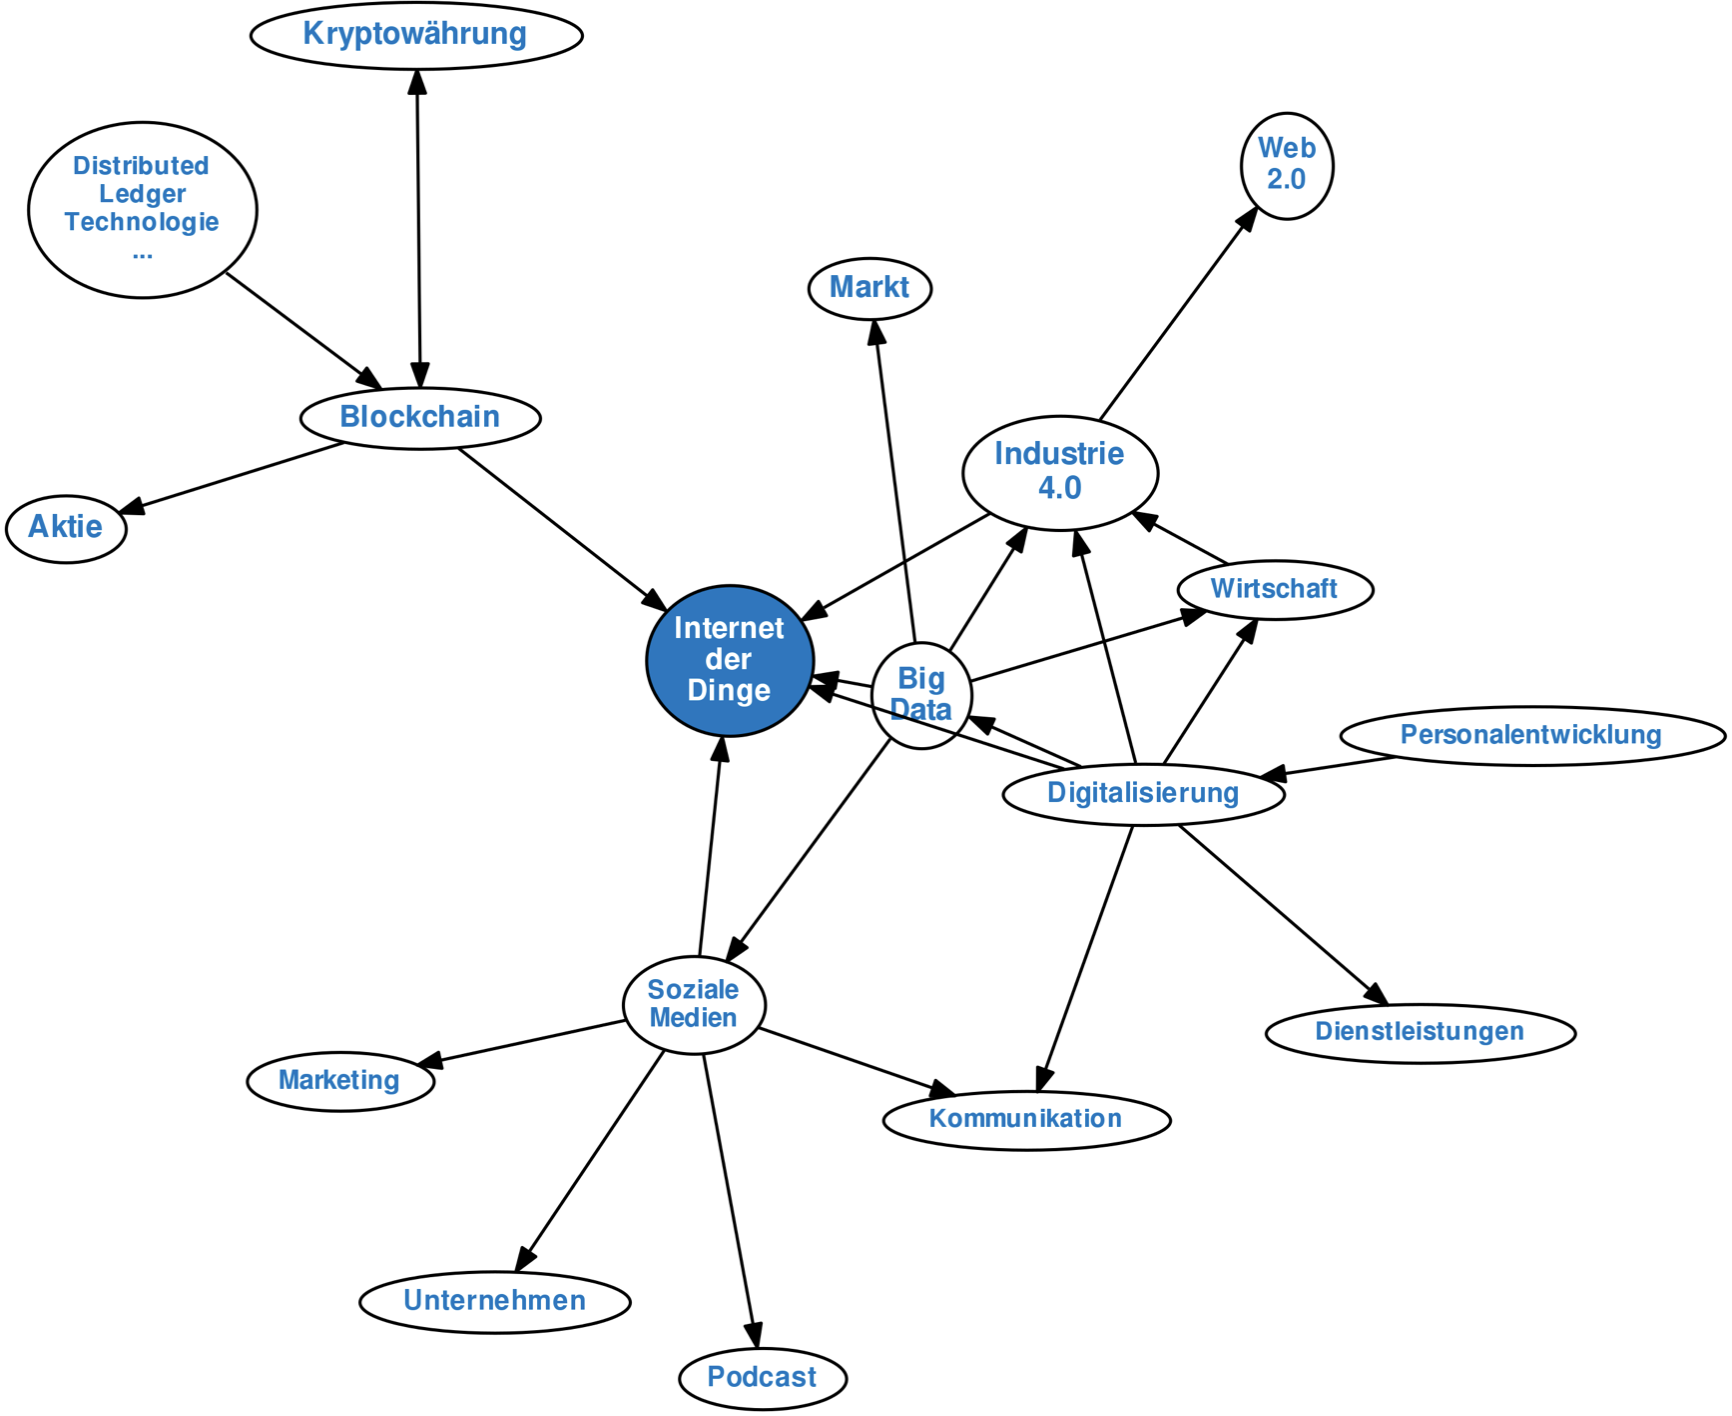
\includegraphics[width=13cm,height=13cm,keepaspectratio]{images/iot_mindmap.png}
        \caption{Technologische Einordnung von IoT \cite{iotmindmap2018}}
        \label{pic:mindmap_IoT}
    \end{figure}




    %\subsection{IIoT}

\subsection{Edge und Cloud Computing}
    %Definition Edge Computing
    %Definition Cloud Computing
    % Unterschiede der beiden Ansätze und in Zusammenhang mit IoT (kurz)

\subsection{Ziele von \acs{IoT}}